\section{Computer programs} % (fold)
\label{sec:computer_programs}

One of the key ideas of reproducible research is that it is a means to communicate not only with colleagues who may wish to understand or to build on our work, but also to communicate with our future selves when we seek to remind ourselves of what we did and how we did it.  Since there is no GitHub repository of the work we did---GitHub not having been invented until 33 years after we started our work---I had to rely on the next best thing, namely, paper files from that era.  Those files are part of my papers that have undergone many moves and many downsizings; it wasn't obvious to me that I would have kept anything of value.  But as it turns out, at least some useful material survived, a testament to the enduring value of paper records, a storage medium and communications format that has survived the test of time.
  
The ET paper relies heavily on computations based on the raw data in Table~1 of ET, reproduced in Figure~\ref{fig:ETT1}, for which custom programs were written, together with some calculations that were apparently done ``by hand'' using the calculator technology of the day.

The main computations appear in Tables~2 through~7.  Table~3 shows maximum likelihood parameter estimates for Fisher's (truncated) negative binomial model for various choices of the truncation parameter, and Table~2 shows the estimated means for word types seen exactly $x$ times calculated from one set of the negative binomial parameters.  Table~4 shows calculated Euler coefficients for the generalized linear vocabulary estimator.  Table~5 contains calculated lower bounds for the expected number of new words that one would see in a body of work $t$ times as large as Shakespeare's extant corpus, and Table~6 shows lower and upper bounds for the same quantities based on a linear programming formulation of the problem.

\begin{figure}
	\centering
	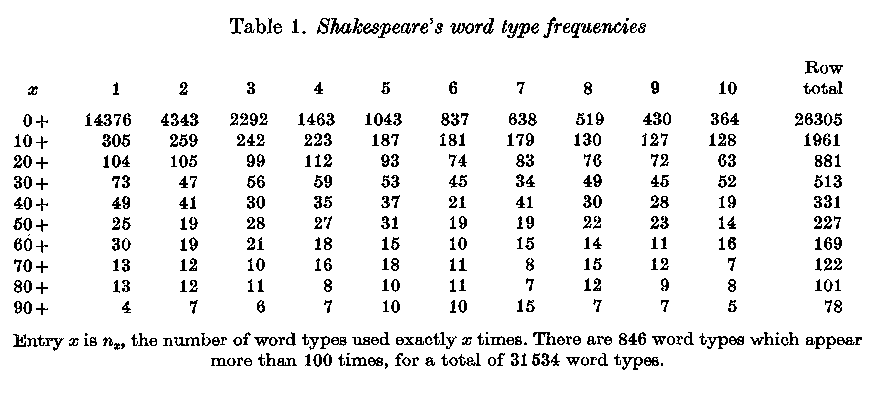
\includegraphics[width=5in]{../compendium/Figures/ET-Table1.pdf}
	\caption{Table~1 from Efron and Thisted \citeyear{Efron:1976zs} }
	\label{fig:ETT1}
\end{figure}

\subsection{Computing circa 1975} % (fold)
\label{sub:computing_circa_1975}
The first task is to determine whether we can replicate the main results, here taken to be the contents of Table~3 from Efron and Thisted \citeyear{Efron:1976zs}\footnote{In this paper we shall focus on the calculations in Tables~2 and~3 to illustrate the issues involved; the calculations of Tables~4 through~6 raise additional difficulties which are beyond the scope of this project; we touch on those issues briefly.}.  These target results are displayed in Figure~\ref{fig:ETT3}

\begin{figure}
	\centering
	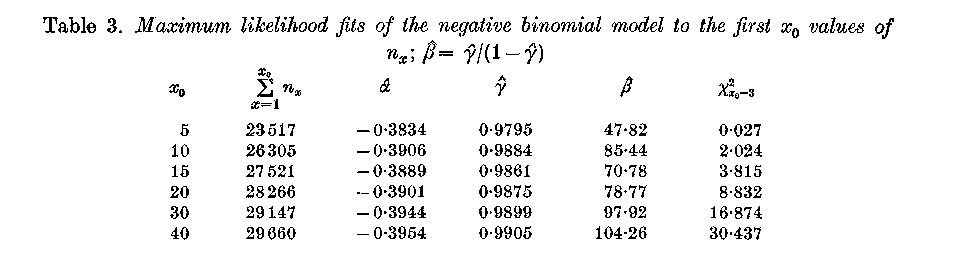
\includegraphics[width=6in]{../compendium/Figures/ET-Table3.pdf}
	\caption{Table~3 from Efron and Thisted \citeyear{Efron:1976zs}.  These are the main results whose reproducibility is at issue. }
	\label{fig:ETT3}
\end{figure}

A starting point is what we did in 1975 when working on our paper.

The computer programs for those calculations used the technology of the day, which in this case involved writing programs in a dialect of BASIC, PL/I, and a script for a IBM proprietary mathematical programming system called MPS/360. As near as I can reconstruct, the PL/I programs were used to generate the input to the MPS software, which was used to solve a large linear optimization program.  IBM discontinued sales and support of MPS in 2005. At the time \texttt{S}, (the statistical programming language that John Chambers developed at Bell Laboratories and the predecessor to \texttt{R}, did not yet exist.  Indeed, there were no general-purposed statistical programming environments on which to draw.

Fortunately, one of us (Thisted) not only seems to have saved large chunks of the working papers from the Shakespeare project, but also to have refrained from tossing them out in the course of multiple relocations and office downsizings.  And I was able to find what may be a program that was used to perform the calculations in Table~3. This program is shown in Figure~\ref{fig:mle-bas-orig}.

\begin{figure}
	\centering
	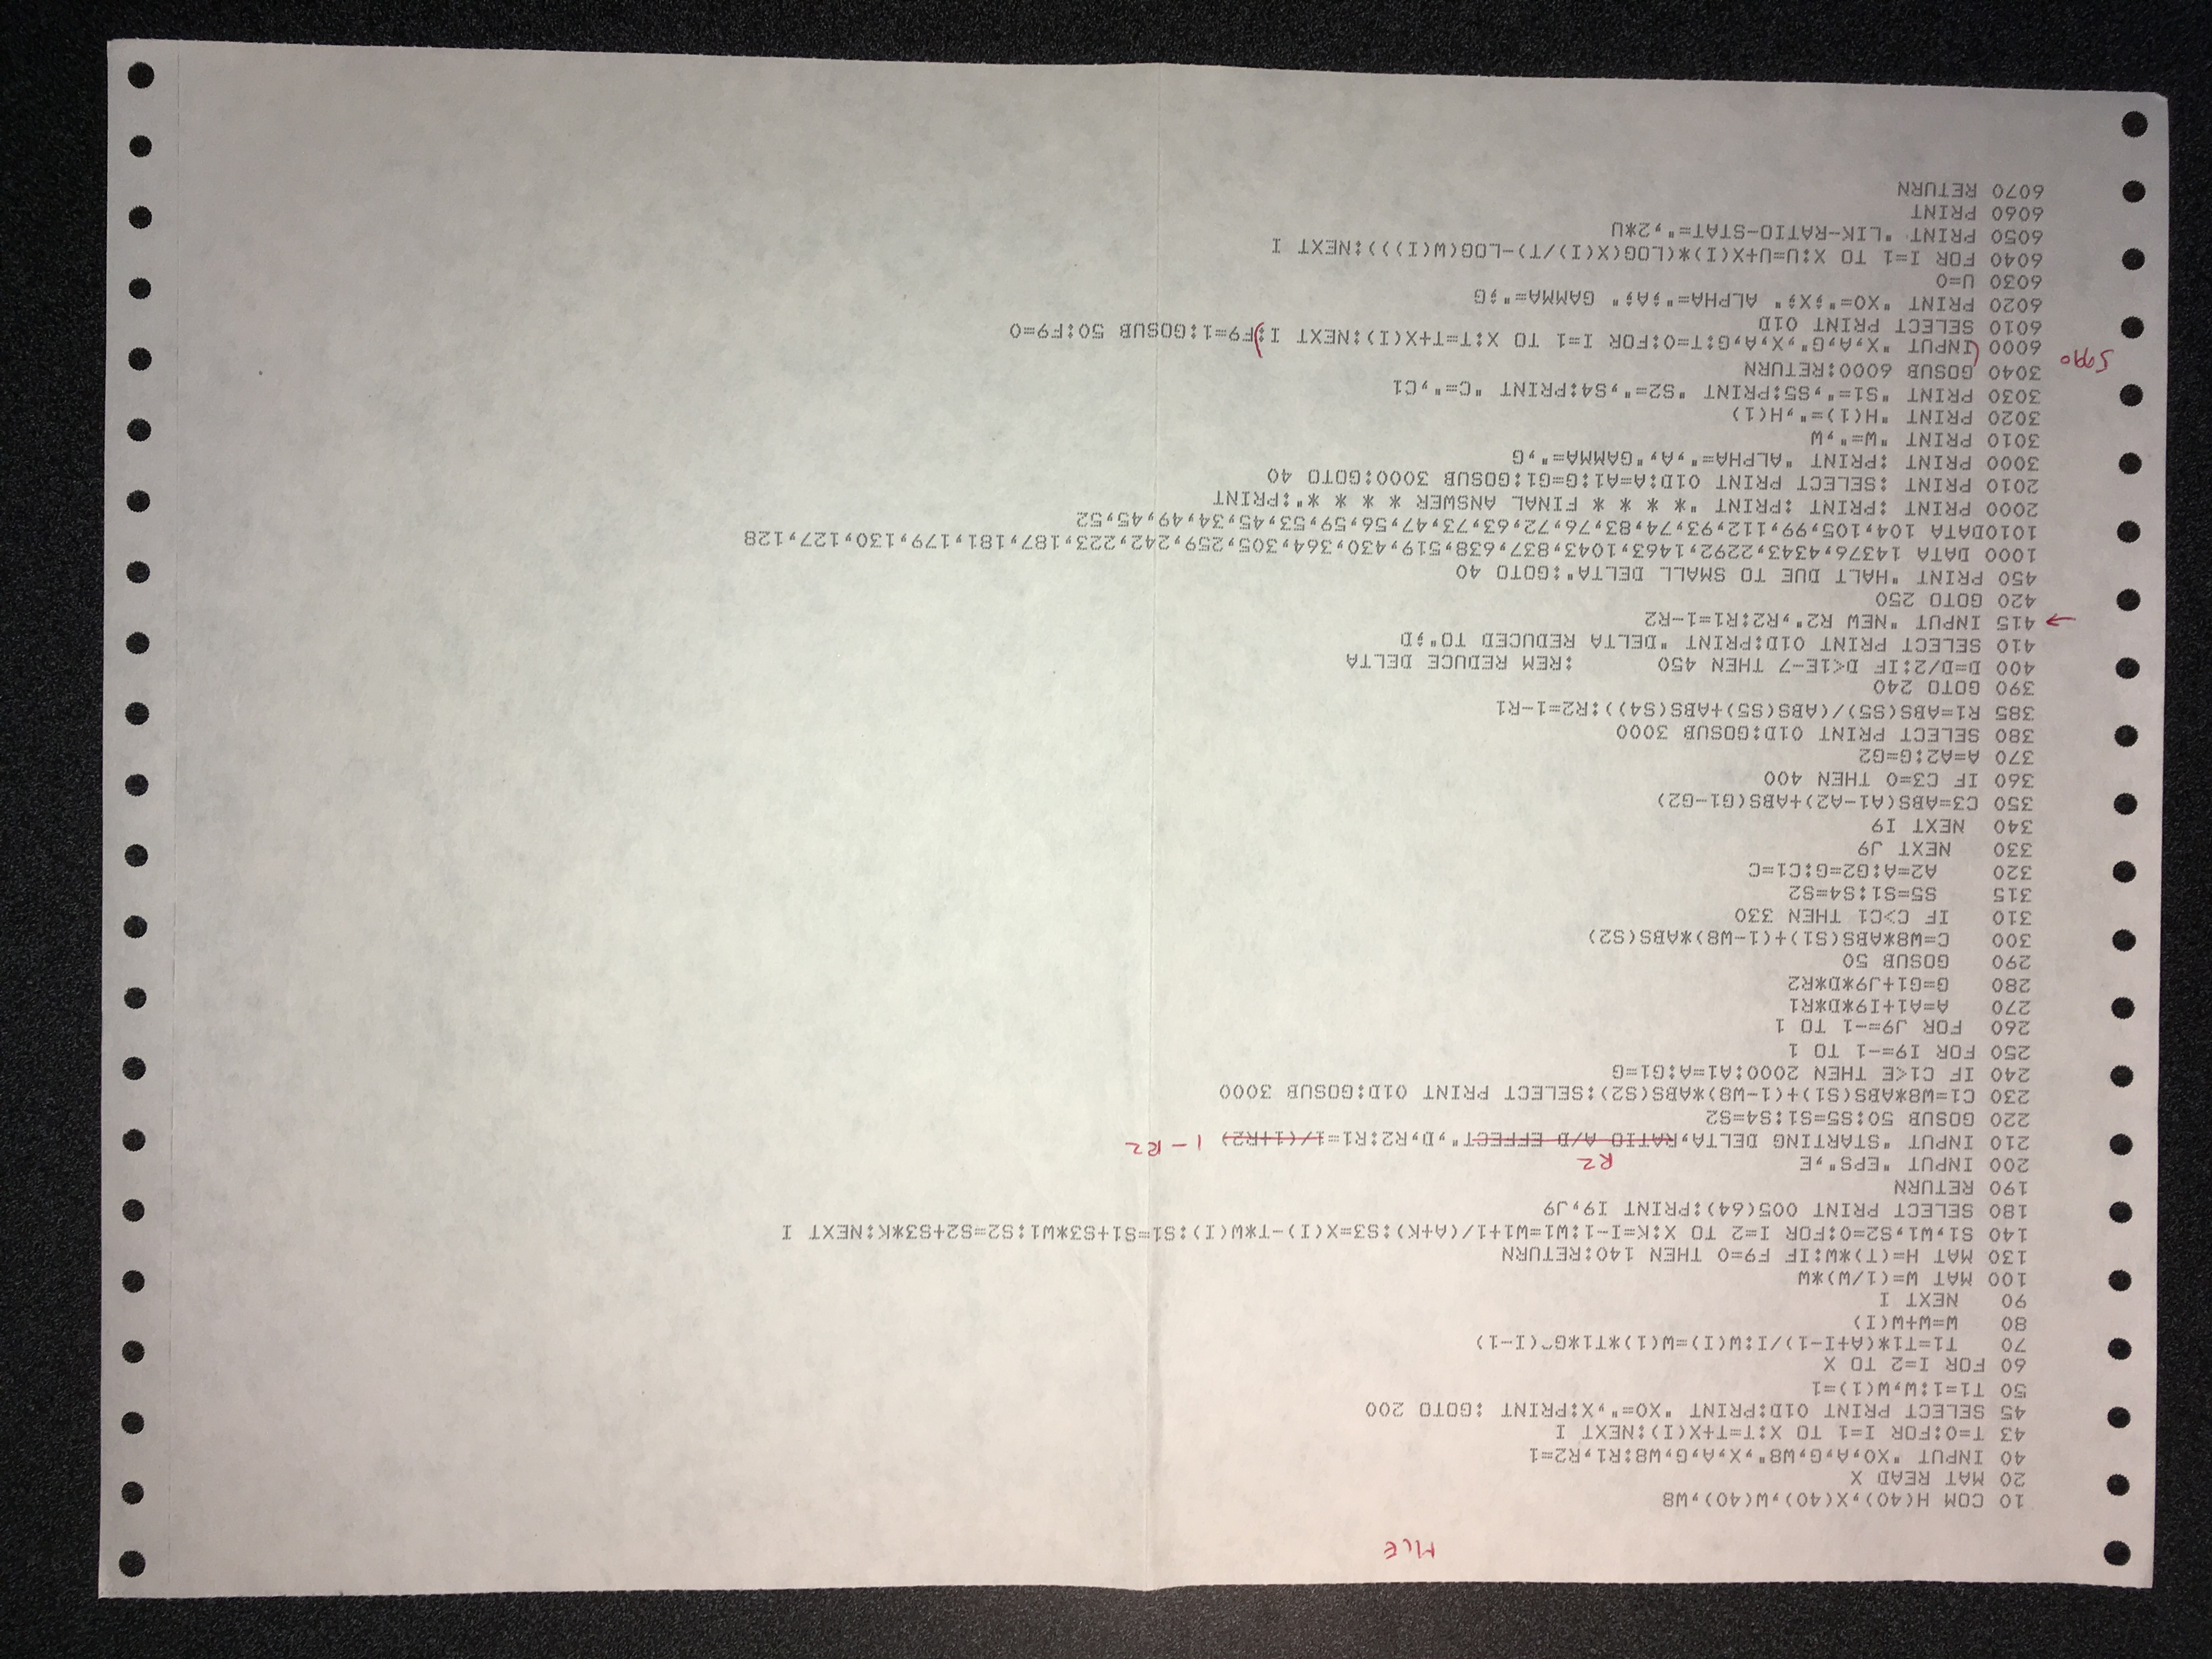
\includegraphics[width=5in,angle=180]{Photos/mle-bas-5036.jpg}
	\caption{Program used to calculate maximum likelihood estimates in Table~3 of Efron and Thisted \citeyear{Efron:1976zs} }
	\label{fig:mle-bas-orig}
\end{figure}

This program was written for the Wang~2200 computer, the departmental computing device of the time, which could be only programmed in this dialect of BASIC.  The program was transcribed, and is included both in Appendix~\ref{cha:basic_mle_program} and in the GitHub repository \texttt{compendium/Programs/mle.bas.txt}.  Unfortunately, there are no Wang~2200s available to me on which I can run this program which, I note, requires manual input of starting values and convergence parameters.

The inputs and outputs to this program were not, unfortunately, among the pieces of papers that I preserved, although one page, shown in Figure~\ref{fig:Table3-output-5037a}, gives a hint, both as to where one set of values (corresponding to $x_0=40$) may have come from, and to how much the process of what actually transpired has been lost.  It is also clear that the output in this figure was not produced by the computer program in Figure~\ref{fig:mle-bas-orig}.  It isn't clear whether the preserved output is from an early prototype of the final program, or the preserved program is an early prototype of the one that produced the output of the latter.

\begin{figure}
	\centering
	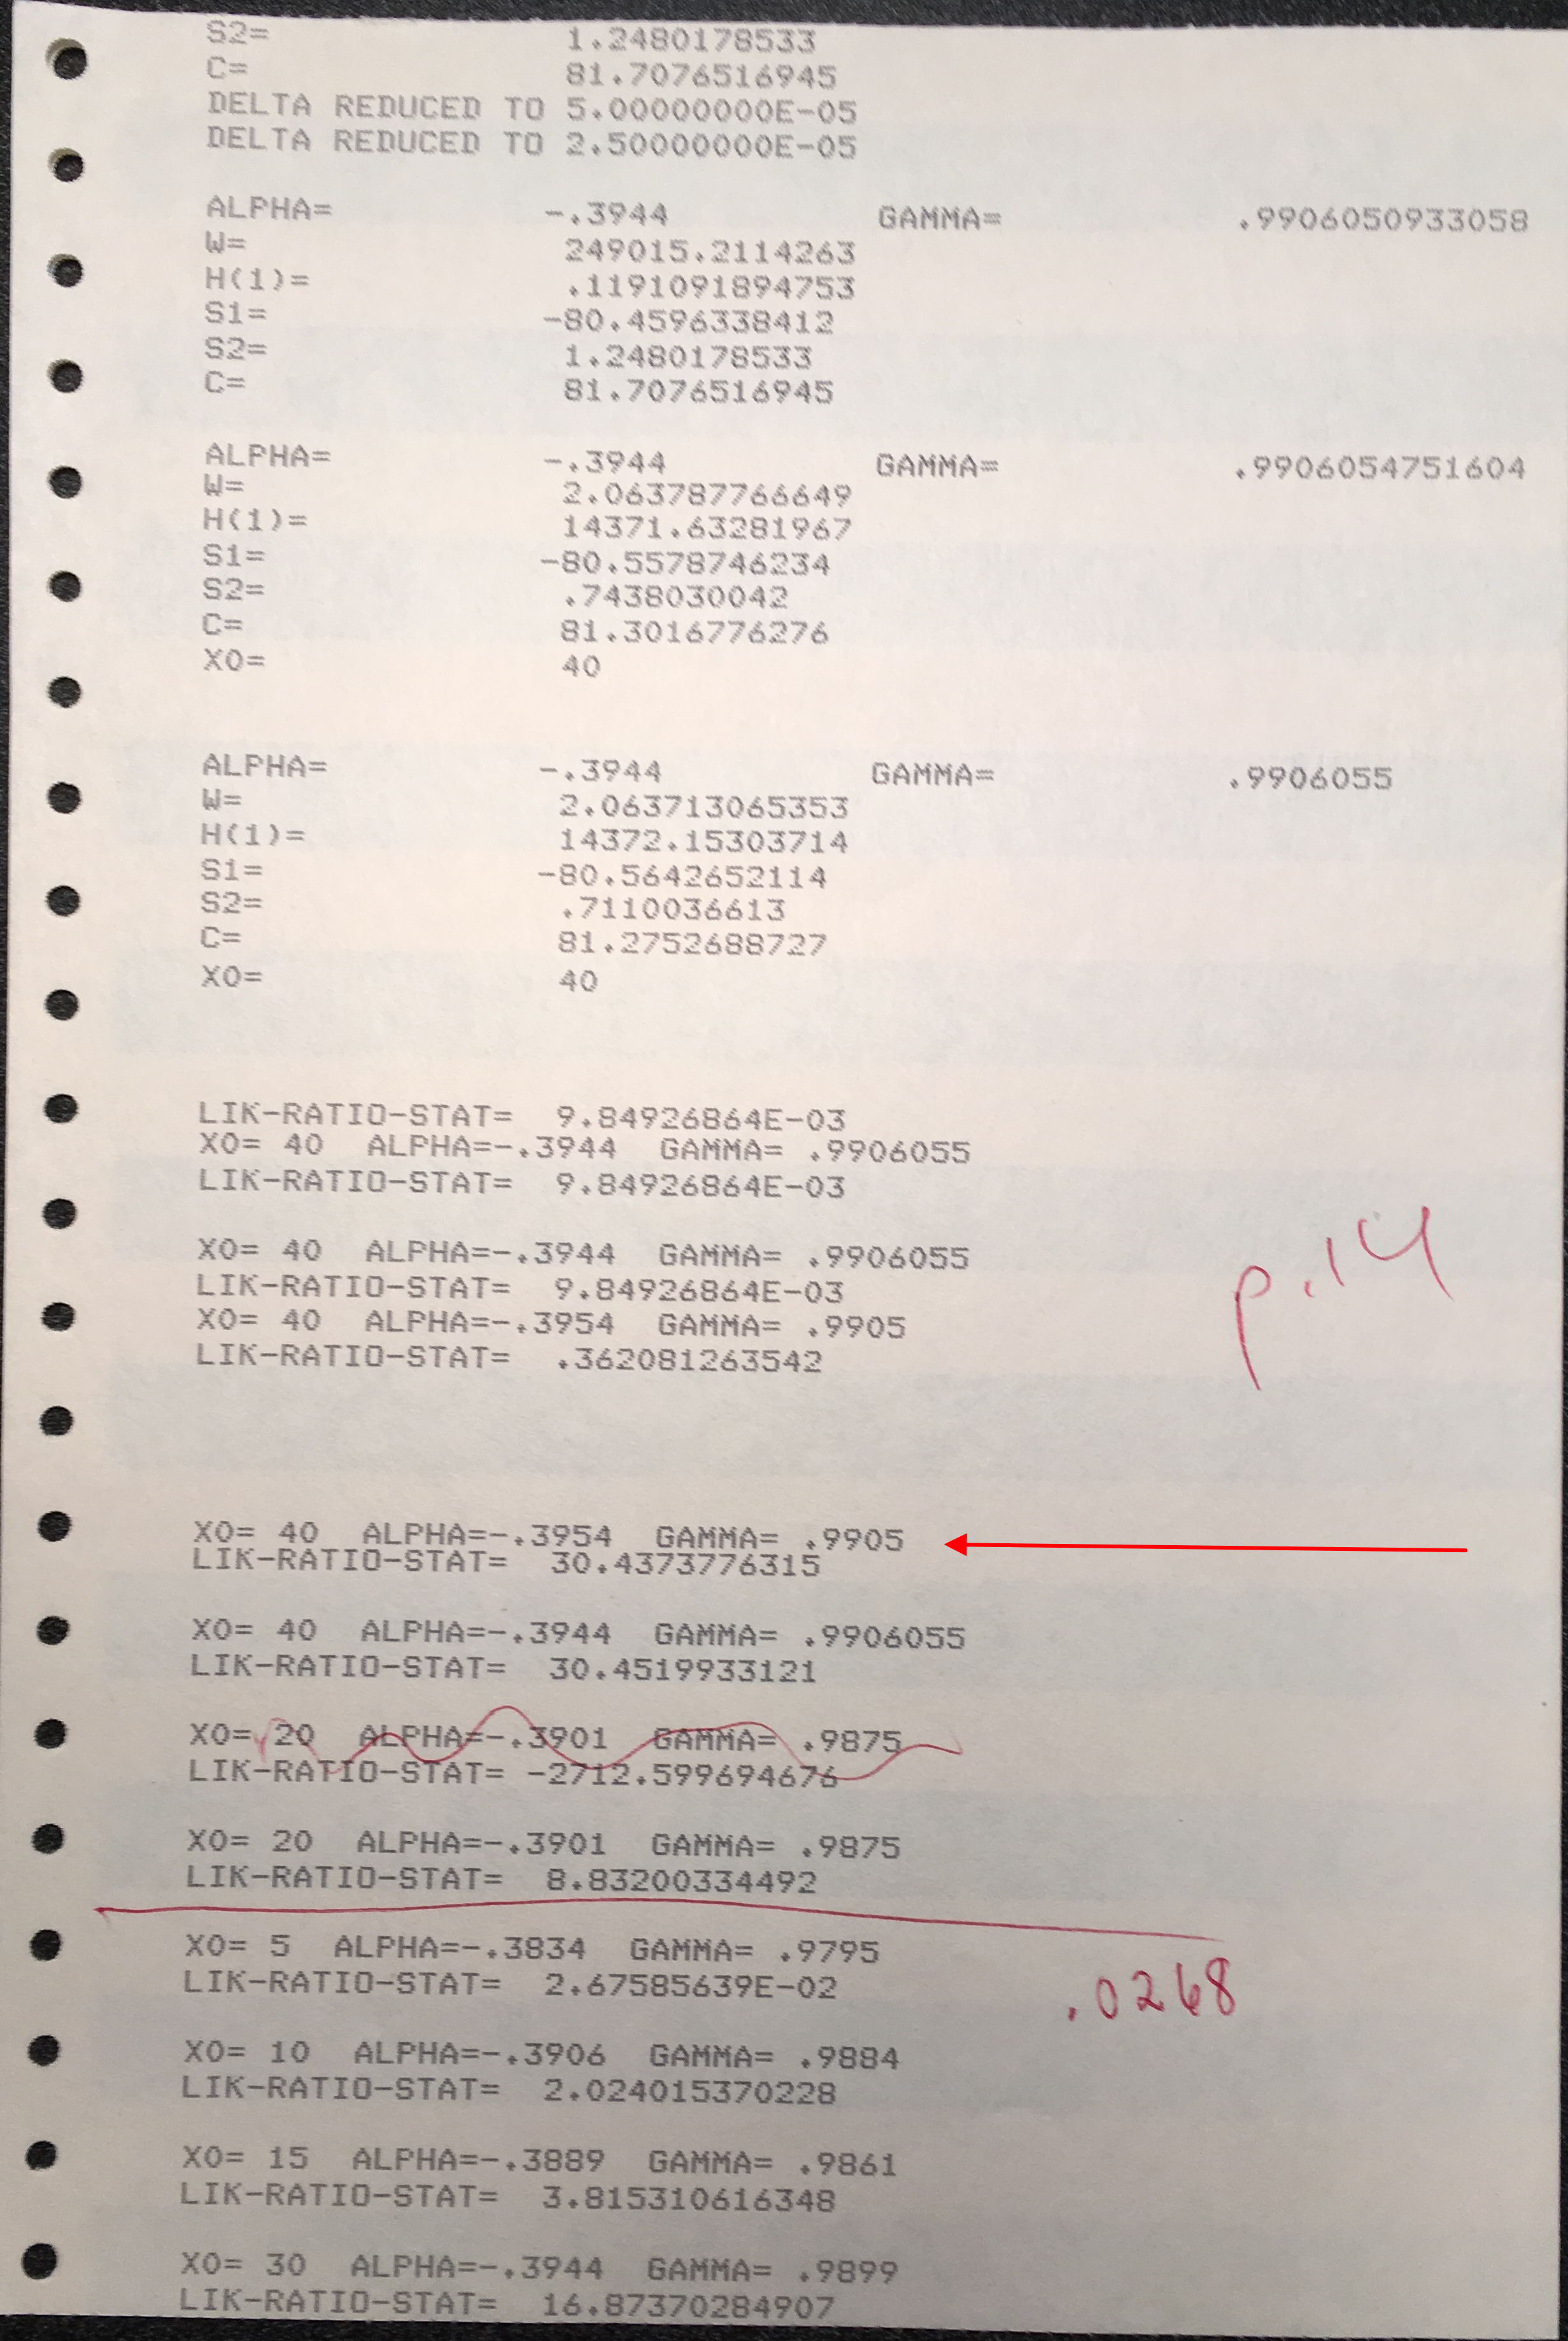
\includegraphics[width=3in]{Photos/Table3-output-5037a.jpg}
	\caption{The apparent source for $\hat\alpha$ and $\hat\gamma$ corresponding to $x_0=40$ in Table~3 of Efron and Thisted \citeyear{Efron:1976zs}.  The red arrow points to the parameter values that appear in the published table. }
	\label{fig:Table3-output-5037a}
\end{figure}

% subsection computing_circa_1975 (end)

\subsection{Recomputing Table~3 from Table~1} % (fold)
\label{sub:recomputing_table_3_from_table_1}

	So how would we do this computation in 2018, and do so in a way that might be more readily reproduced 40~years hence than our work from 40~years ago seems to have been?  The first step is to determine just what model is being fit.  Although the paper itself isn't crystal clear on the point, the model corresponding to $x_0$ is simply fitting a multinomial with $x_0$ categories (corresponding to $x=1$ through $x_0$), the probability $p_x$ for category $x$ being proportional to
$$
p_x \propto {\Gamma(x+\alpha) \over x! \Gamma(1+\alpha)}\gamma^{x-1},
$$
for $\gamma<1$ and $\alpha>-1$, and where $n_x$ is the number of word types observed in category $x$.  The trickiness in the calculation results from the ``proportional to'' description of the probabilities, as the proportionality factor that ensures the probabilities sum to unity itself is a function of the parameters. 
	
	In response to one of the recent queries about how we got the values in Table~3, I resorted to the quickest (and dirtiest) method possible: I used the black-box optimizer built into Excel!  This spreadsheet (\texttt{ET-Table3-origdata.xlsx}, locked 12:36pm CDT 12 May 2018) is available in the GitHub repository for those interested.  This required building a separate pane for each choice of $x_0$, in which the calculations were performed.  The results analogous to ET's Table~3 are in the Summary pane, and are reproduced in Table~\ref{tab:excel}.
	
\begin{table}
	\centering
	\begin{tabular}{rrrrrr}
$x_0$ & $\sum n_x$ & $\hat\alpha$ & $\hat\gamma$ & $\hat\beta$ & $\chi_{x_0-3}^2$\\[3mm]
 5  & 23517  & -0.3834 &  0.9795 &   47.71 &   0.027\\
10  & 26305  & -0.3902 &  0.9883 &   84.48 &   2.024\\
15  & 27521  & -0.3867 &  0.9854 &   67.42 &   3.752\\
20  & 28266  & -0.3894 &  0.9872 &   77.20 &   8.822\\
30  & 29147  & -0.3945 &  0.9899 &   98.18 &  16.873\\
40  & 29660  & -0.3973 &  0.9912 &  112.22 &  30.437\\
\end{tabular}


	\caption{Maximum likelihood estimates calculated using Microsoft Excel's built-in optimizing routine.}\label{tab:excel}
\end{table}

	A comparison of Table~3 from ET shown in Figure~\ref{fig:ETT3} and the results from Excel in Table~\ref{tab:excel} shows reasonably good agreement, although there are a few things to note.  First, the results for $\hat\alpha$ agree in the first two decimal places, but diverge in the third, with the greatest divergence for $x_0=40$.  Second, the $\chi^2$ values for the Excel calculation are always less than or equal to those of the original calculation.  This suggests that Excel is actually finding a slightly larger value for the maximized log likelihood.  Third, although the $\chi^2$ values are identical at $x_0=40$, the values for both $\hat\alpha$ and $\hat\gamma$ differ in the third decimal place, which suggests that the likelihood function is relatively flat in the neighborhood of the solution.
	
	Of course if the goal is to maximize reproducibility in the future, an Excel spreadsheet is very nearly the worst possible choice.  Such spreadsheets are easily corrupted by accident, provide no method for documenting changes, and are opaque as to computing formul\ae\ and processes.

	Today there are many well-supported programming environments with high-quality numerics and descriptive scripting languages that make even  non-standard problems like that of fitting the Fisher negative binomial model relatively straightforward to solve.  For purposes of recreating Table~3, I used Stata \citeyear{StataCorp:2017aa}, a computer package widely used by epidemiologists, biostatisticians, and econometricians, since it has a general-purpose maximum likelihood capability.  Stata also has a strong focus on both the quality of the numerical algorithms it employs and on documentation of those algorithms, so using Stata affords a comparison with the black-box, unscripted Excel spreadsheet.
	
	Solving the problem in Stata involves two scripts.  The first contains a program that calculates log-likelihood values that Stata's built in maximum likelihood program (\texttt{ml}) calls when it is run; the second is the wrapper for the calculation that invokes the \texttt{ml} command as applied to the model at hand.  These scripts are reproduced in Appendices~\ref{cha:stata_negative_binomial_log_likelihood} and~\ref{cha:stata_table_3_reproduction} (as well as the GitHub repository at \texttt{compendium/Analysis/et.do} and \texttt{compendium/Analysis/table3mlFromTable1.do}, respectively.)  Both scripts include the line ``\texttt{version 15.1}'', which ensures that should the script be run under later versions of Stata, it will be executed under the rules prevailing under version~15.1.
	
	The results from running the Stata script are given in Table~\ref{table:Stata}, which also includes a line for $x_0=100$, a set of values that we did not calculate in~1975.
	
\begin{table}
	\centering
	\input{StataMLE-Table3-origdata}
	\caption{Maximum likelihood estimates calculated using Stata's \texttt{ml} program for maximum likelihood calculation, coupled with the user-written likelihood specification script \texttt{et.do}.}\label{table:Stata}
\end{table}
	
	The Stata-based results agree very well with those from the Excel spreadsheet, with values for $\hat\gamma$ being identical between the two, and values for $\hat\alpha$ differing by no more than one unit in the fourth decimal place.  Stata also provides asymptotic standard errors for the parameters.

% subsection recomputing_table_3_from_table_1 (end)

% section computer_programs (end)
